\section{SIMULATION RESULTS}

\subsection{BLOCK DIAGRAM OF THE SYSTEM}

\begin{figure}[H]
	\centering
	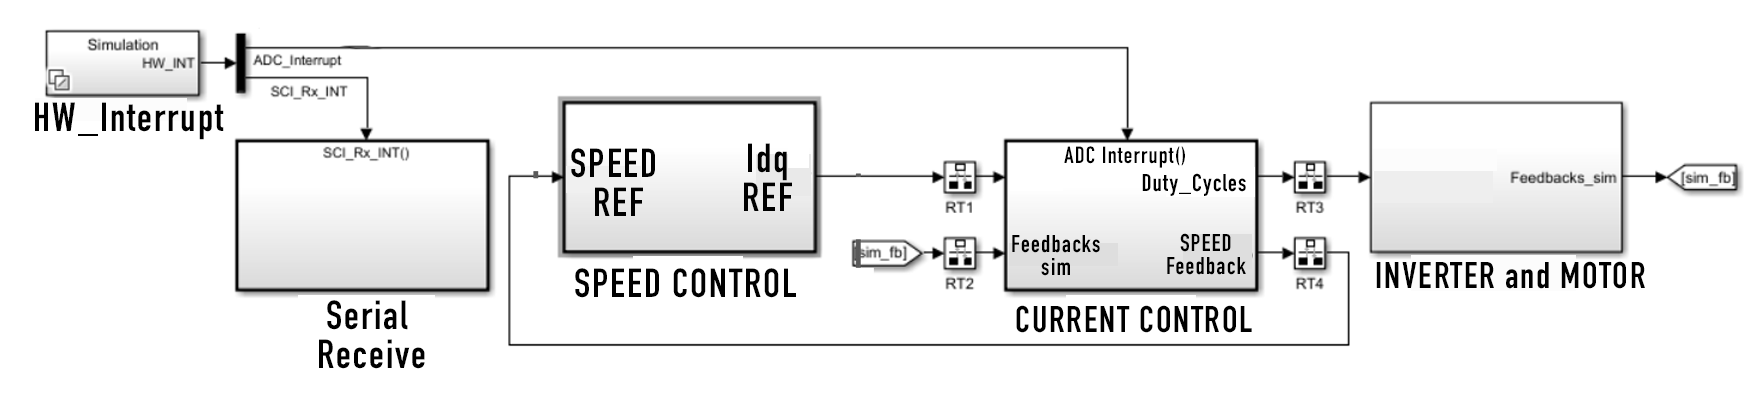
\includegraphics[width=6in]{sections/section3/images/simulation/blockDia.png}
	\caption{Block Diagram of the System}
	\label{fig:block_diagram}
\end{figure}


\subsection{SPEED CONTROL SUBSYSTEM}

\begin{figure}[H]
	\centering
	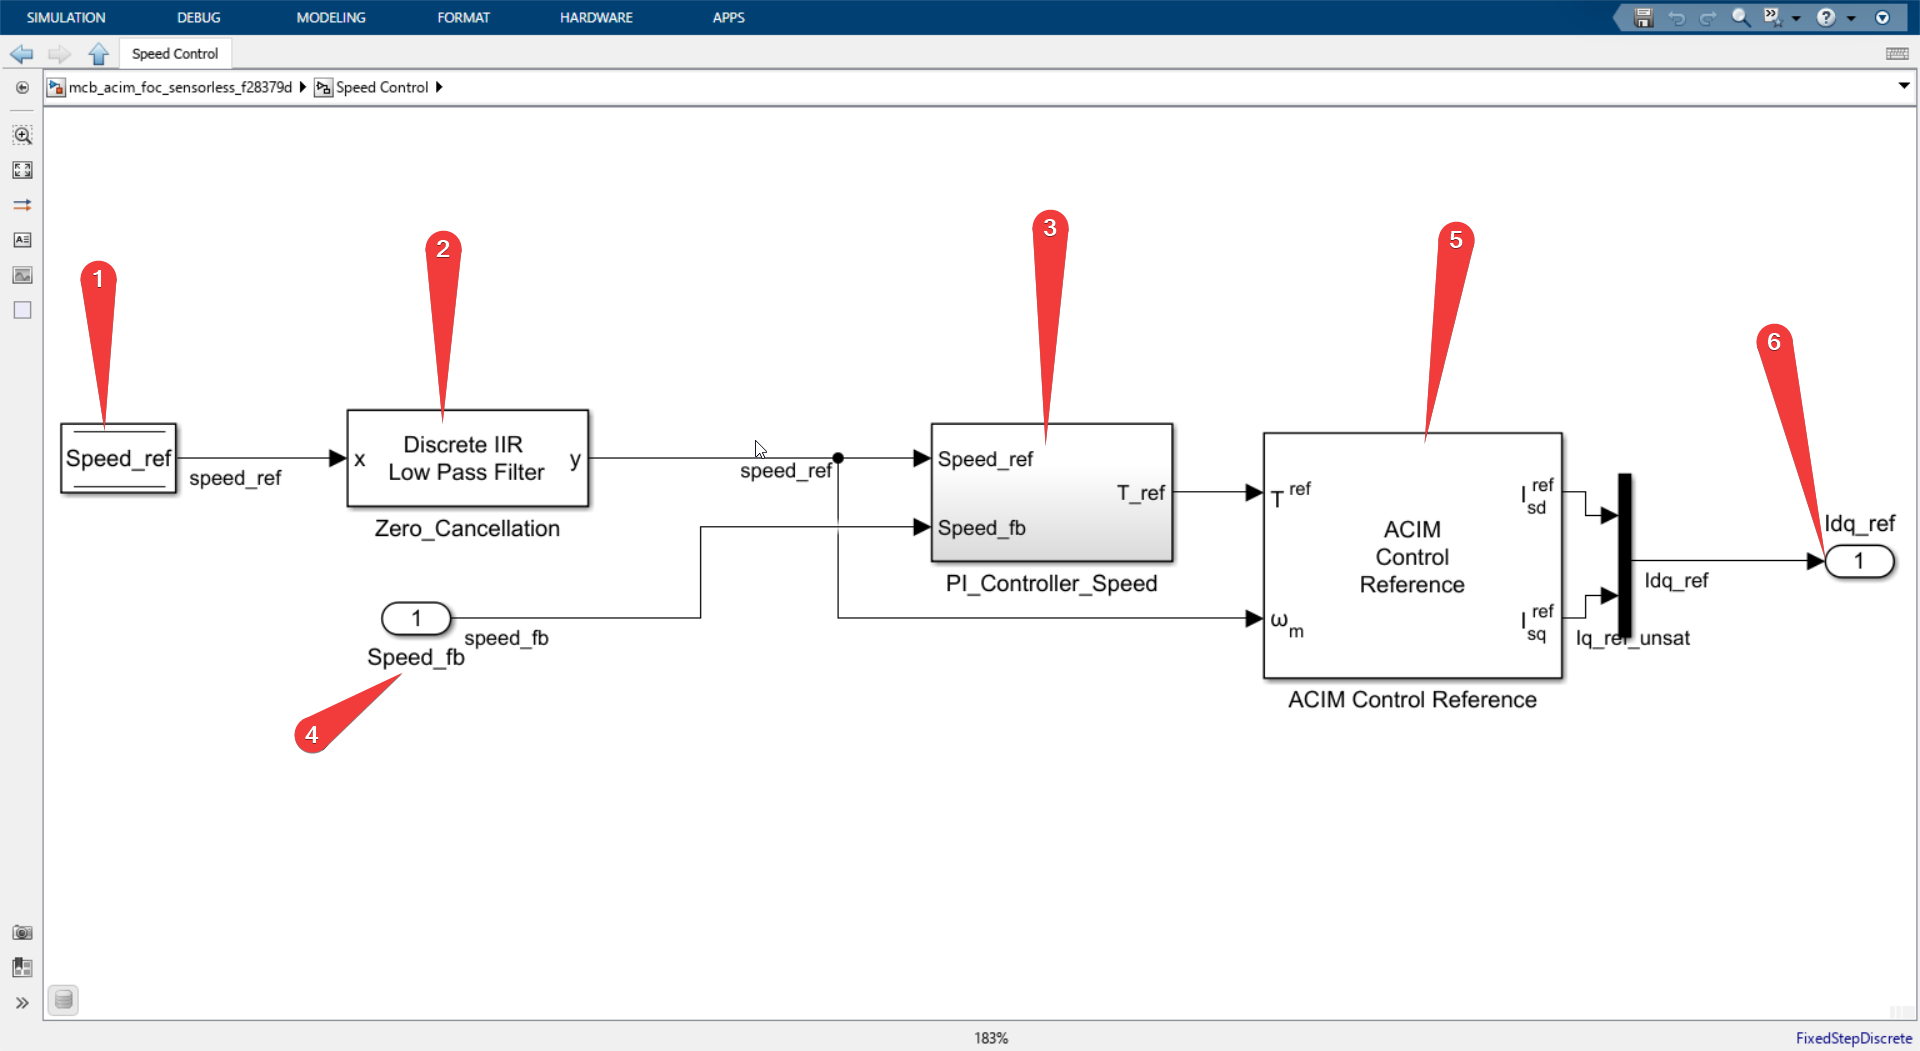
\includegraphics[width=4in]{sections/section3/images/simulation/speedControl/speedController.png}
	\caption{Speed Control System}
	\label{fig:speed_control_system}
\end{figure}


The speed control system shown in Figure \ref{fig:speed_control_system} consists of a DataStoreRead block that holds the speed reference value received from the host computer, a Discrete IIR lowpass filter block to cancel the zeros in the system, and a Discrete PID Controller with anti-windup block that takes the speed reference and feedback values as inputs and generates the torque reference as output. The ACIM Control reference block then takes the torque reference and speed reference as inputs and generates the $Isd_{ref}$ and $Isq_{ref}$ values, which are the reference values for the current control loop. The DQ limiter block is used to limit the magnitude of the vector represented in the d-q reference frame, with the option to prioritize either the d-axis or q-axis component.


\subsection{CURRENT CONTROL SUBSYSTEM}

\subsubsection{CURRENT MEASUREMENT}


\begin{figure}[H]
	\centering
	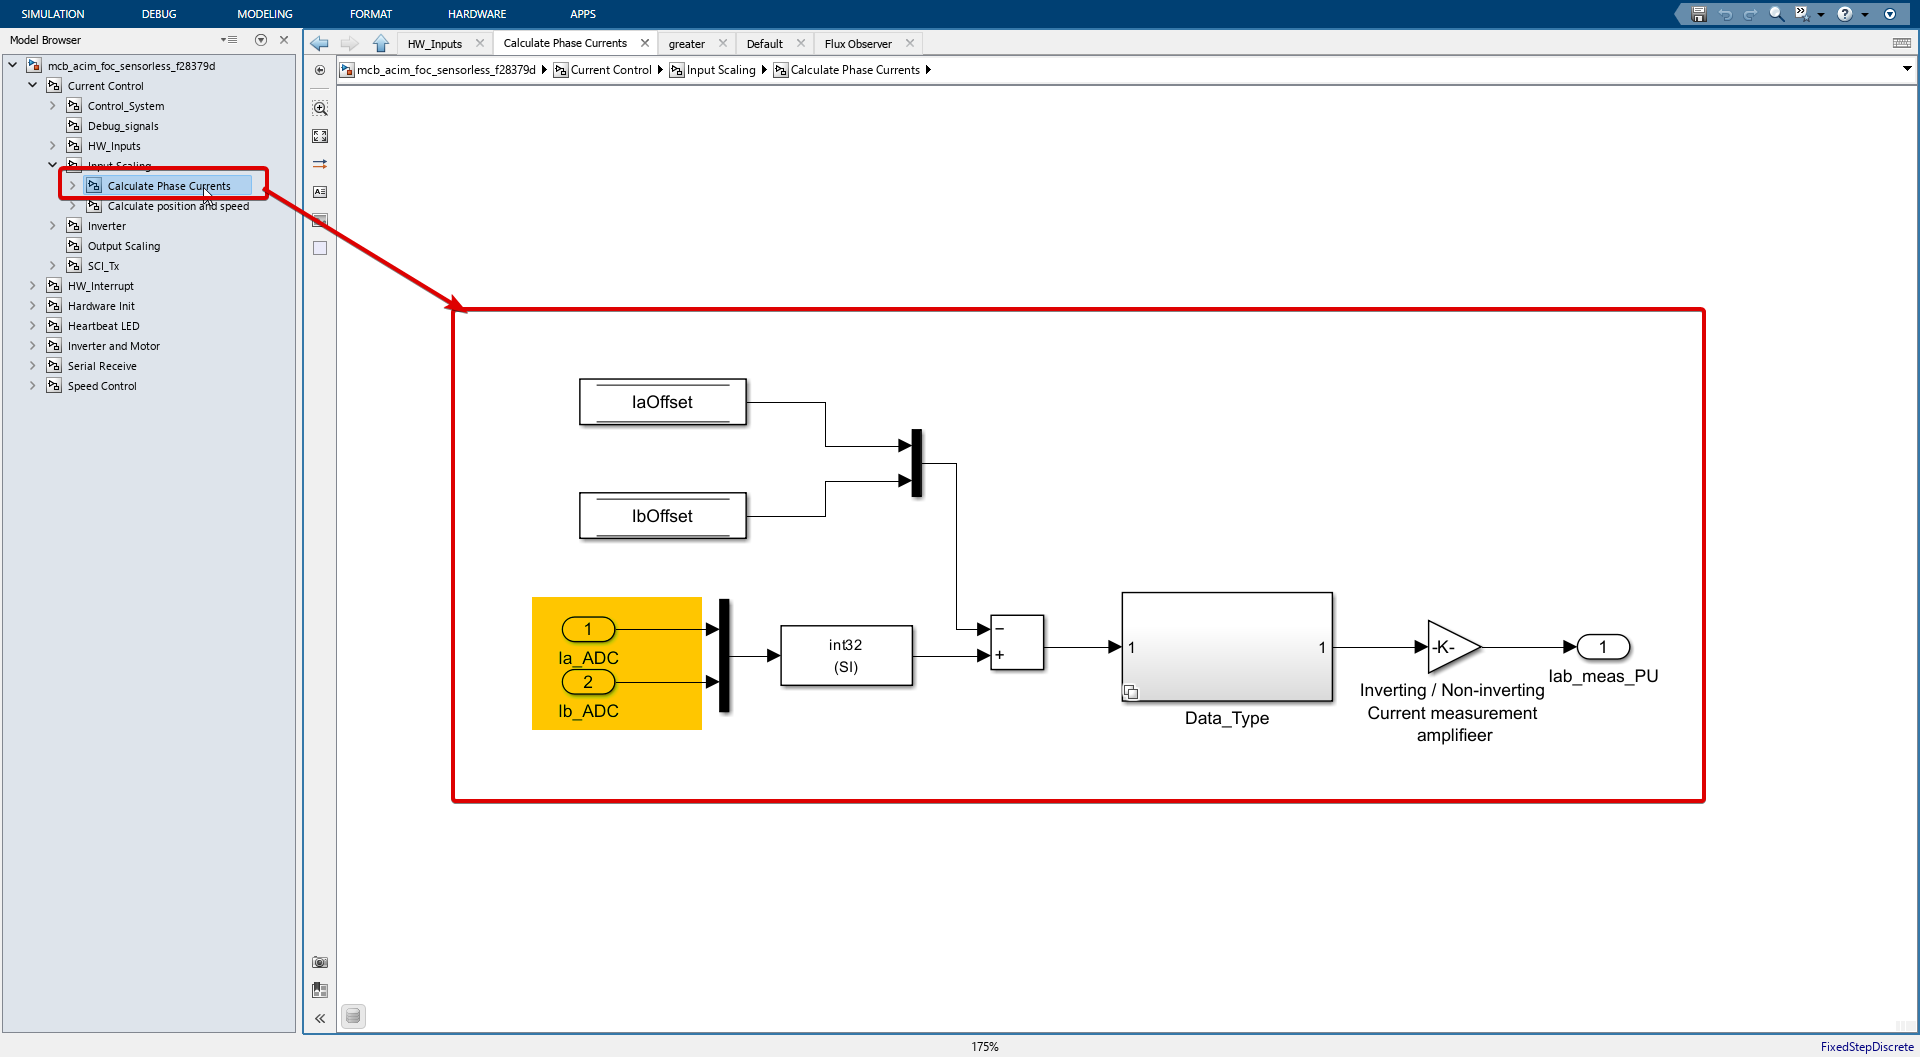
\includegraphics[width=4in]{sections/section3/images/simulation/inputScaling/currentMeasurement.png}
	\caption{Current Measurement}
	\label{fig:current_measurement}
\end{figure}


The current measurement part of the Input Scaling block shown in Figure \ref{fig:current_measurement}

converts the $Ia_{ADC}$ and $Ib_{ADC}$ inputs from the ADCs to the appropriate data type (int32) and removes the offsets ($Ia_{offset}$ and $Ib_{offset}$) that were previously calibrated. The signals then go through a series of gain blocks to convert them to per-unit (PU) values. The first gain block converts the ADC voltage to the actual voltage, the second gain block converts the voltage to current using the inverter's current sense voltage per amp, and the third gain block converts the current to PU using the motor's base current.


\subsubsection{POSITION AND SPEED ESTIMATION}



\begin{figure}[H]
	\centering
	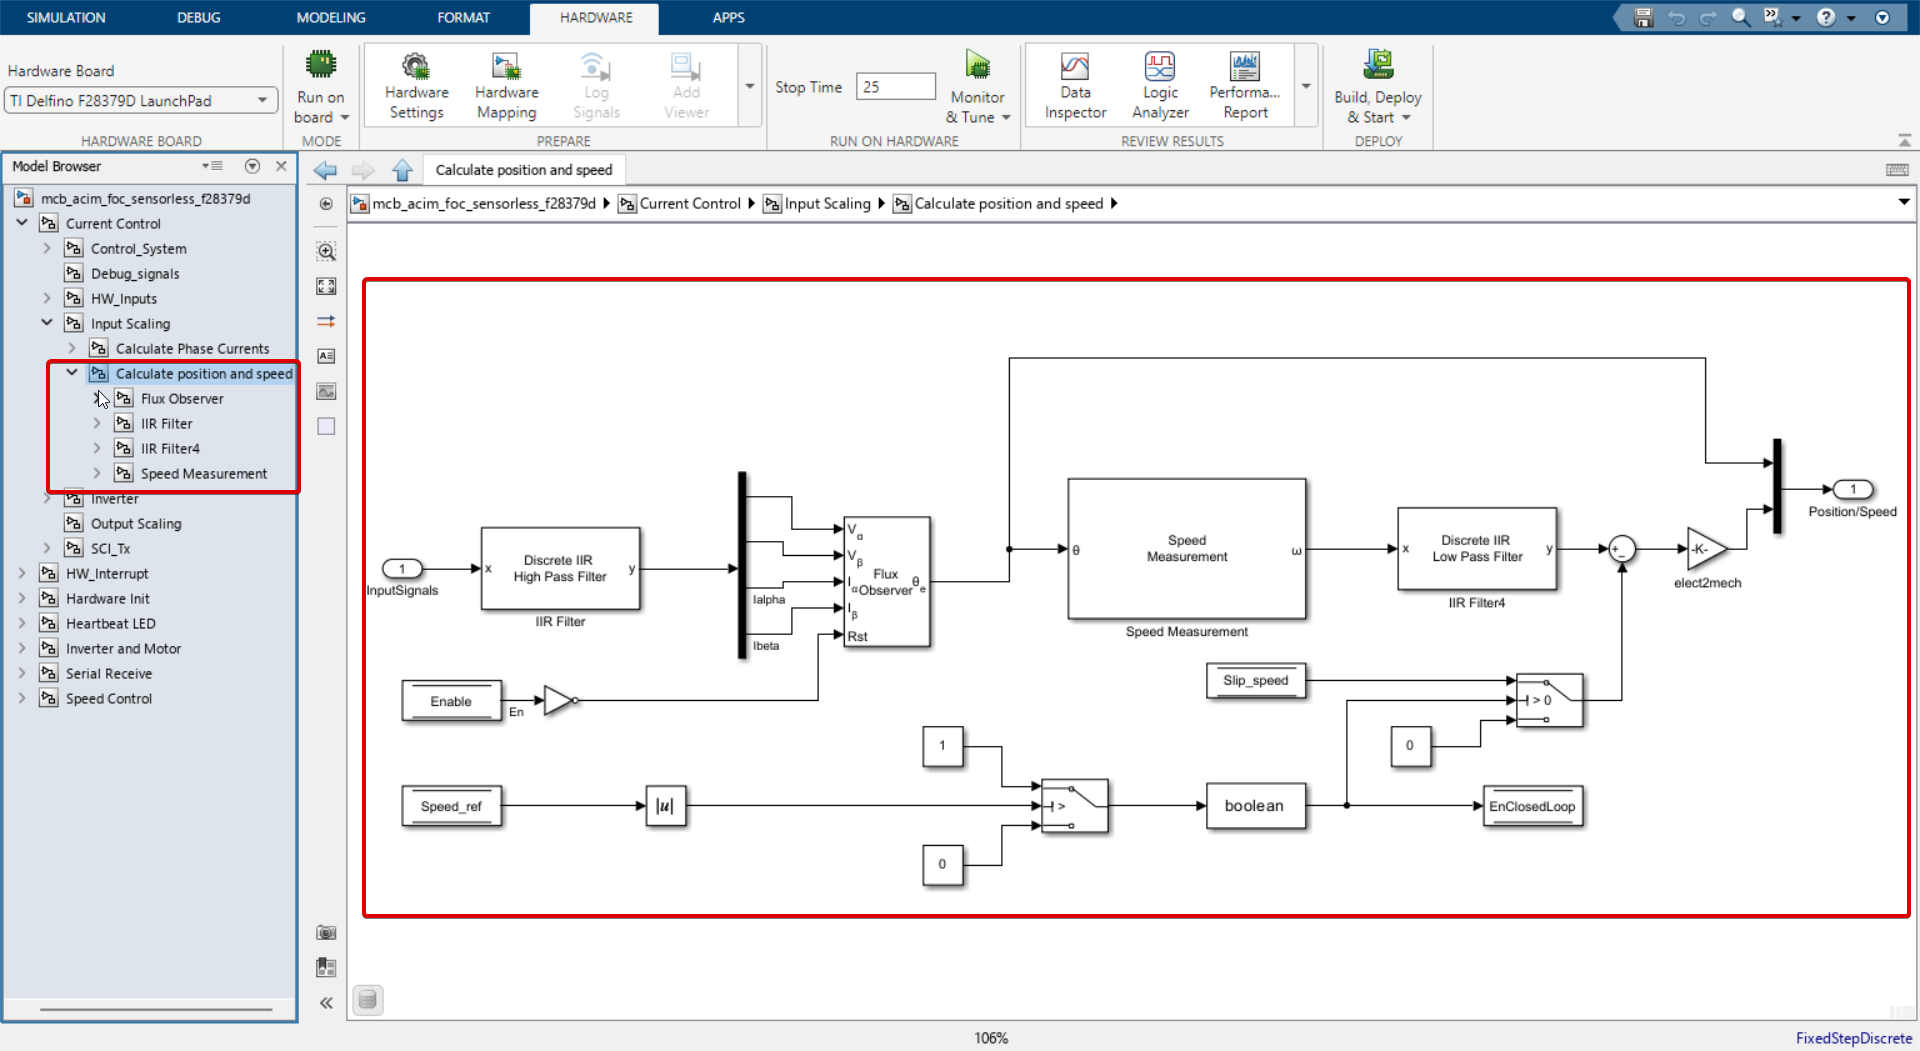
\includegraphics[width=4in]{sections/section3/images/simulation/inputScaling/fluxObserver.png}
	\caption{Position and Speed Estimation}
	\label{fig:position_speed_estimation}
\end{figure}


The position and speed estimation part of the Input Scaling block shown in  Figure \ref{fig:position_speed_estimation} uses the $VI_{fb}$ signal, which contains the motor's voltage and current in the $\alpha \beta$ reference frame. This signal goes through a high-pass filter to remove low-frequency noise. The filtered signals are then fed into the Flux Observer block, which estimates the stator flux position. The estimated stator flux position is then used in the Speed Estimation block to calculate the motor's speed. The estimated speed is filtered using a low-pass IIR filter to remove high-frequency noise. The final rotor speed is calculated by subtracting the slip speed from the estimated stator flux speed and then dividing by the number of pole pairs to get the mechanical speed.

\subsubsection{CONTROL SYSTEM}



\begin{figure}[H]
	\centering
	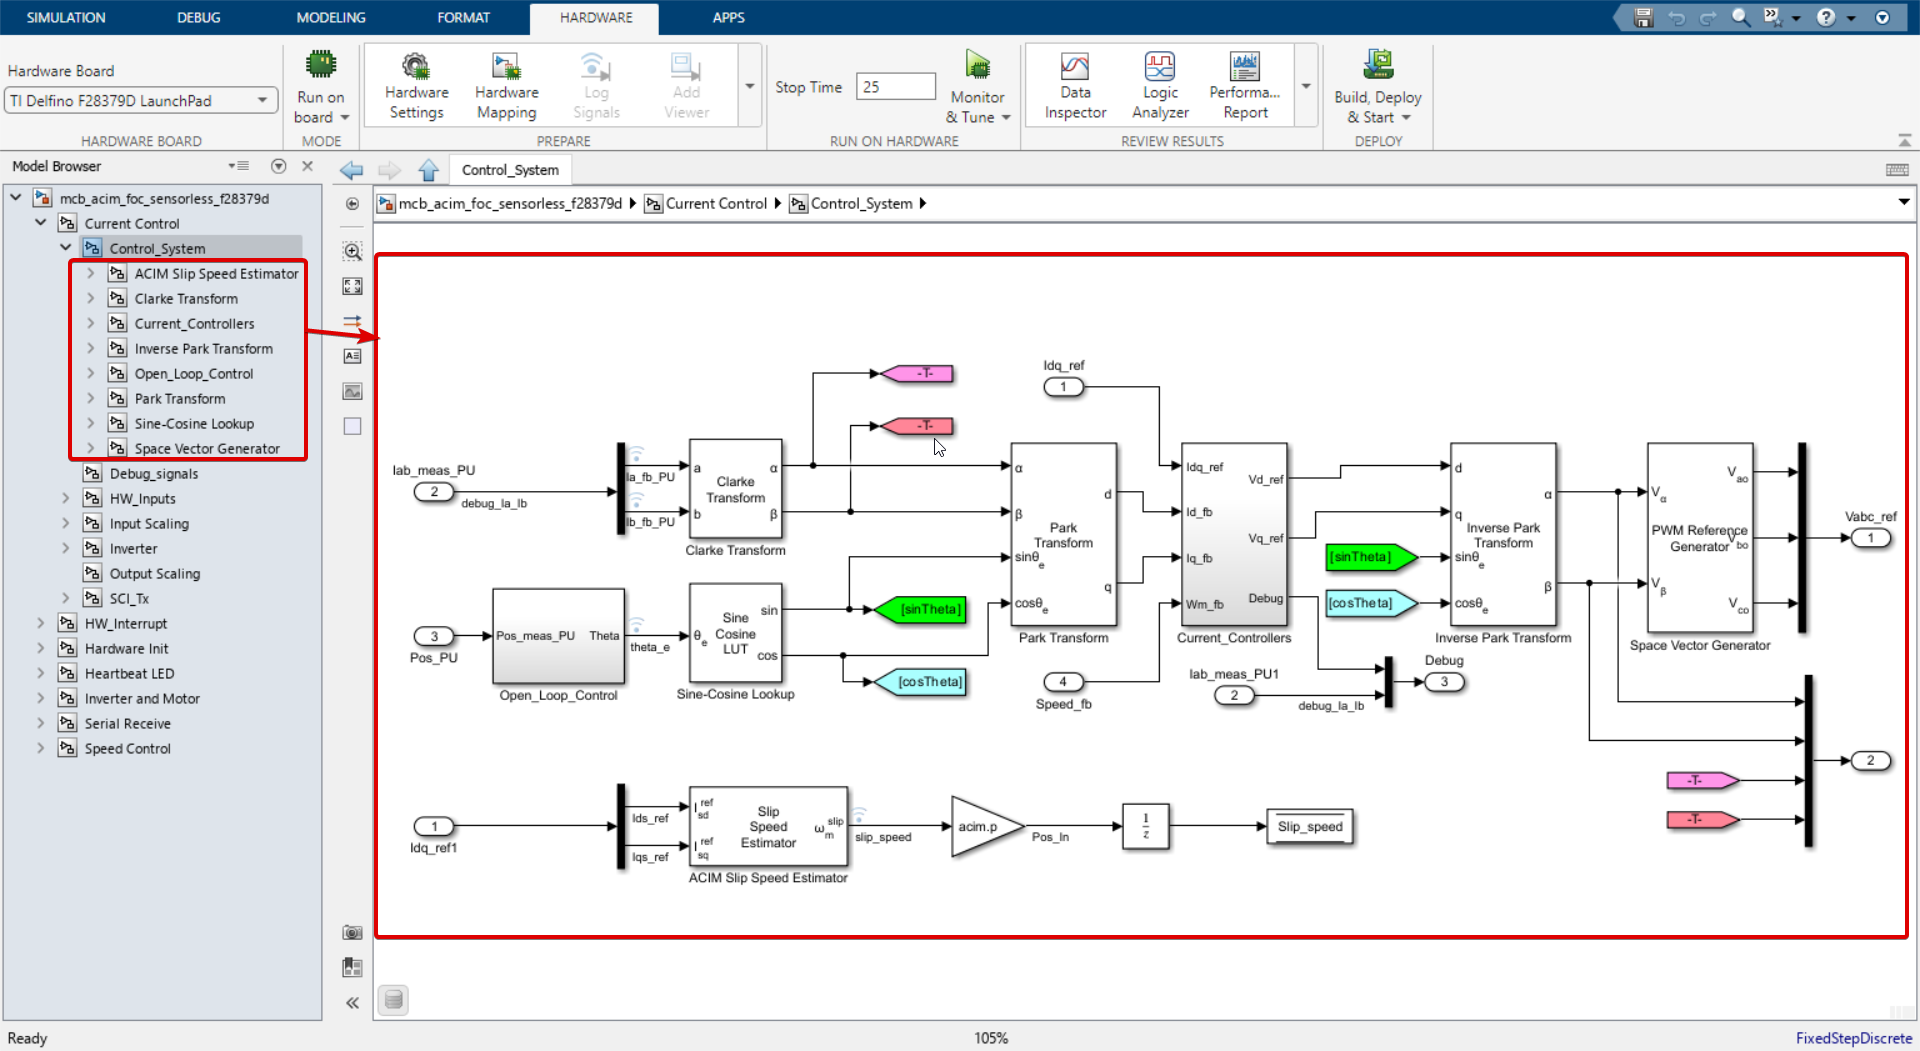
\includegraphics[width=4in]{sections/section3/images/simulation/currentControl/controlSystem.png}
	\caption{Current Control System}
	\label{fig:current_control_system}
\end{figure}


The control system shown in Figure \ref{fig:current_control_system} implemented in the inner current loop consists of two main components: the current controllers and the DQO transformation.

The current controllers use Proportional-Integral (PI) controllers to minimize the error between the reference currents ($I_{dq\_{ref}}$) and the feedback currents ($I_{d\_fb}$ and $I_{q\_fb}$). The output of the PI controllers is then limited, filtered, and adjusted using a feedforward controller and a saturation function to ensure safe and reliable operation of the system. The adjusted d-axis current is then used to generate the reference voltages ($V_{d\_{ref}}$ and $V_{q\_{ref}}$) in the DQ frame. These reference voltages are then transformed into the alpha-beta frame using the stator flux position ($\theta$) and fed into the PWM reference generator block, which generates the three-phase voltage references for the inverter. This inner current loop ensures that the actual currents closely follow the desired reference currents, which is crucial for the overall performance and stability of the control system.



\subsection{SIMULATION RESULTS}

\subsubsection{SPEED RESPONSE}

\begin{figure}[H]
	\centering
	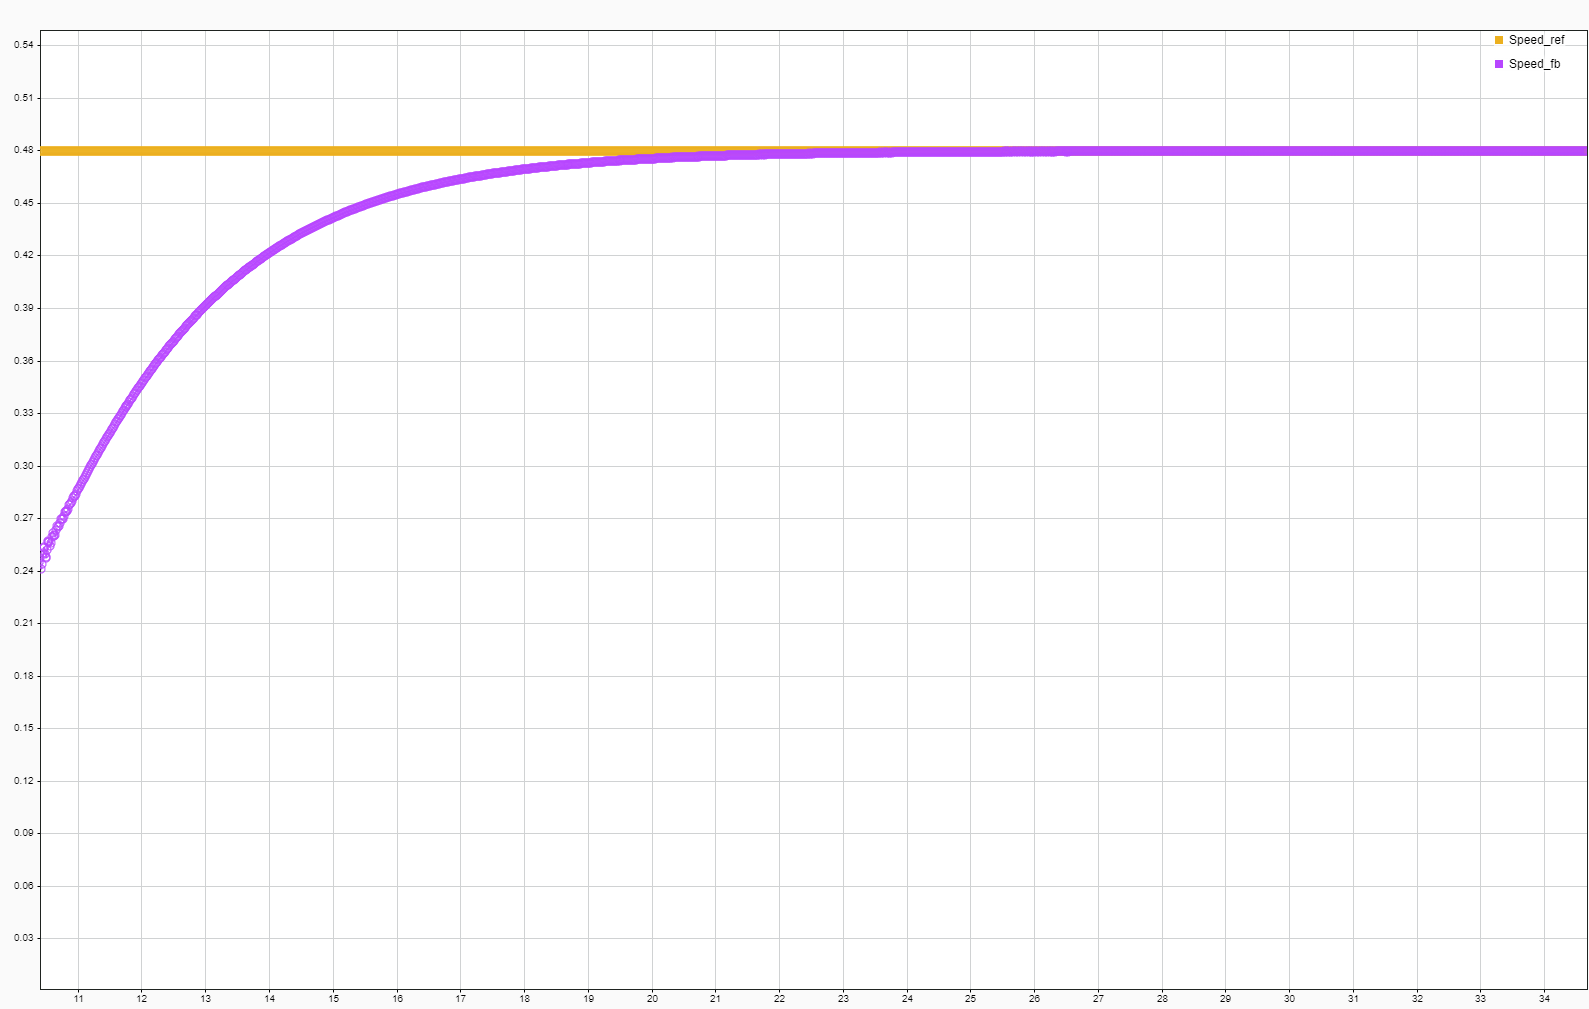
\includegraphics[width=6in]{sections/section3/images/simulationResutls/SpeedTrackingNoCursor.png}
	\caption{Speed Response}
	\label{fig:speed_response}
\end{figure}


\begin{figure}[H]
	\centering
	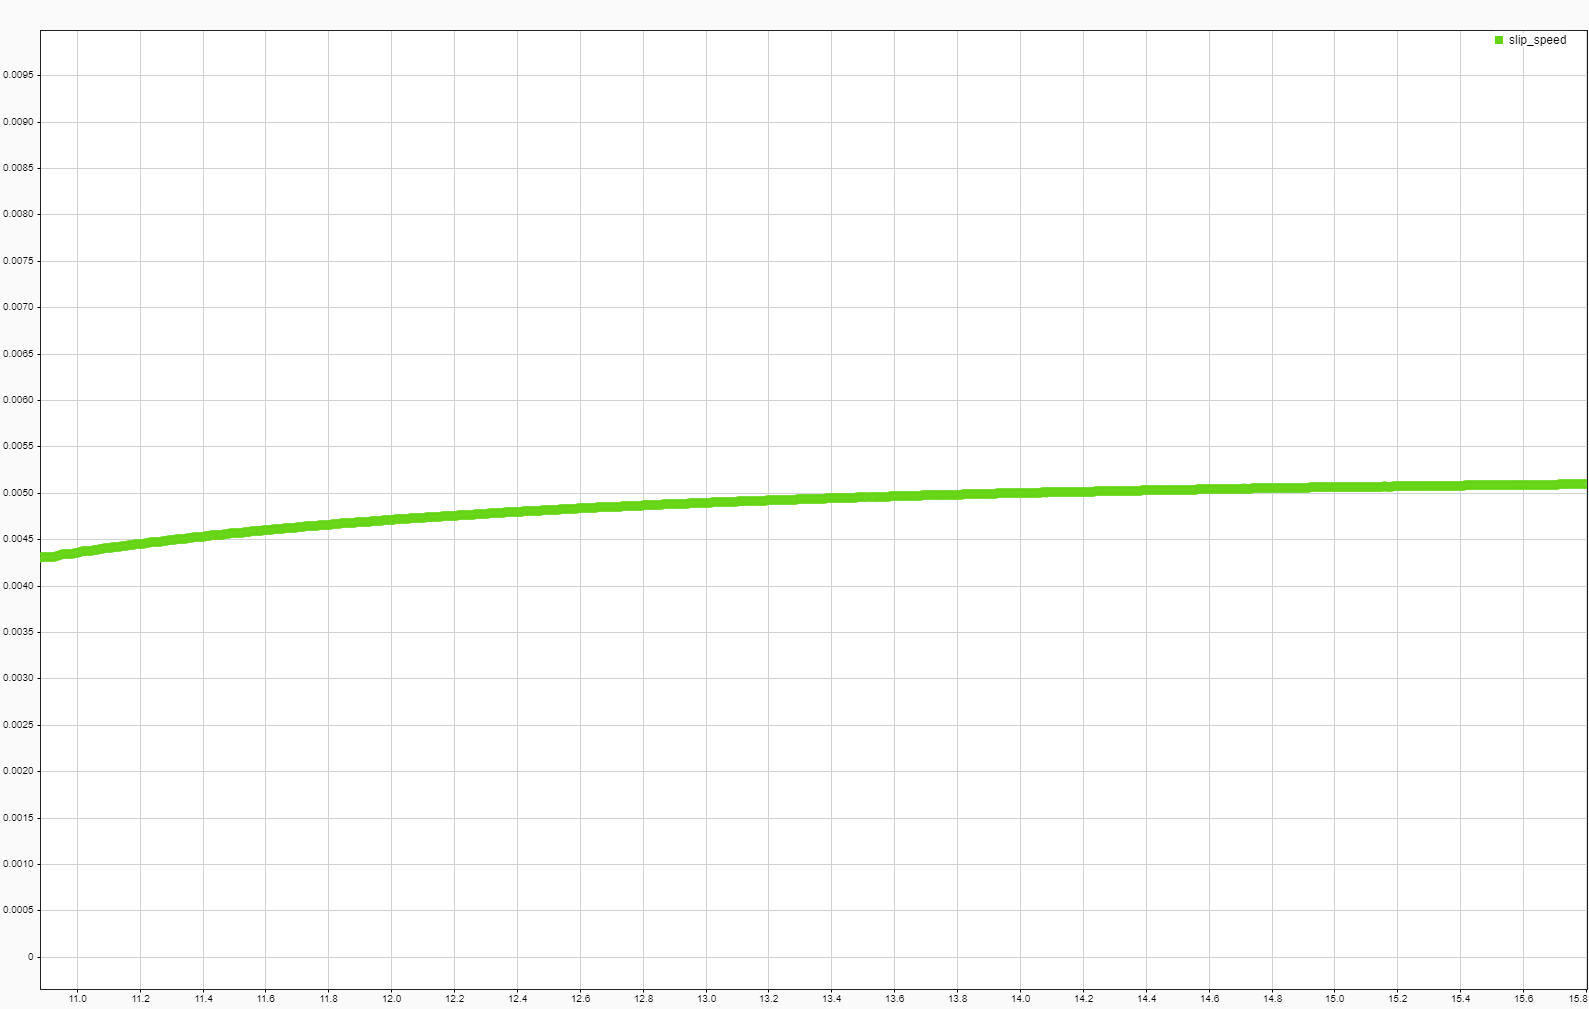
\includegraphics[width=6in]{sections/section3/images/simulationResutls/SlipSpeed.png}
	\caption{Slip Speed}
	\label{fig:slip_speed}
\end{figure}

\subsubsection{CURRENT RESPONSE}


\begin{figure}[H]
	\centering
	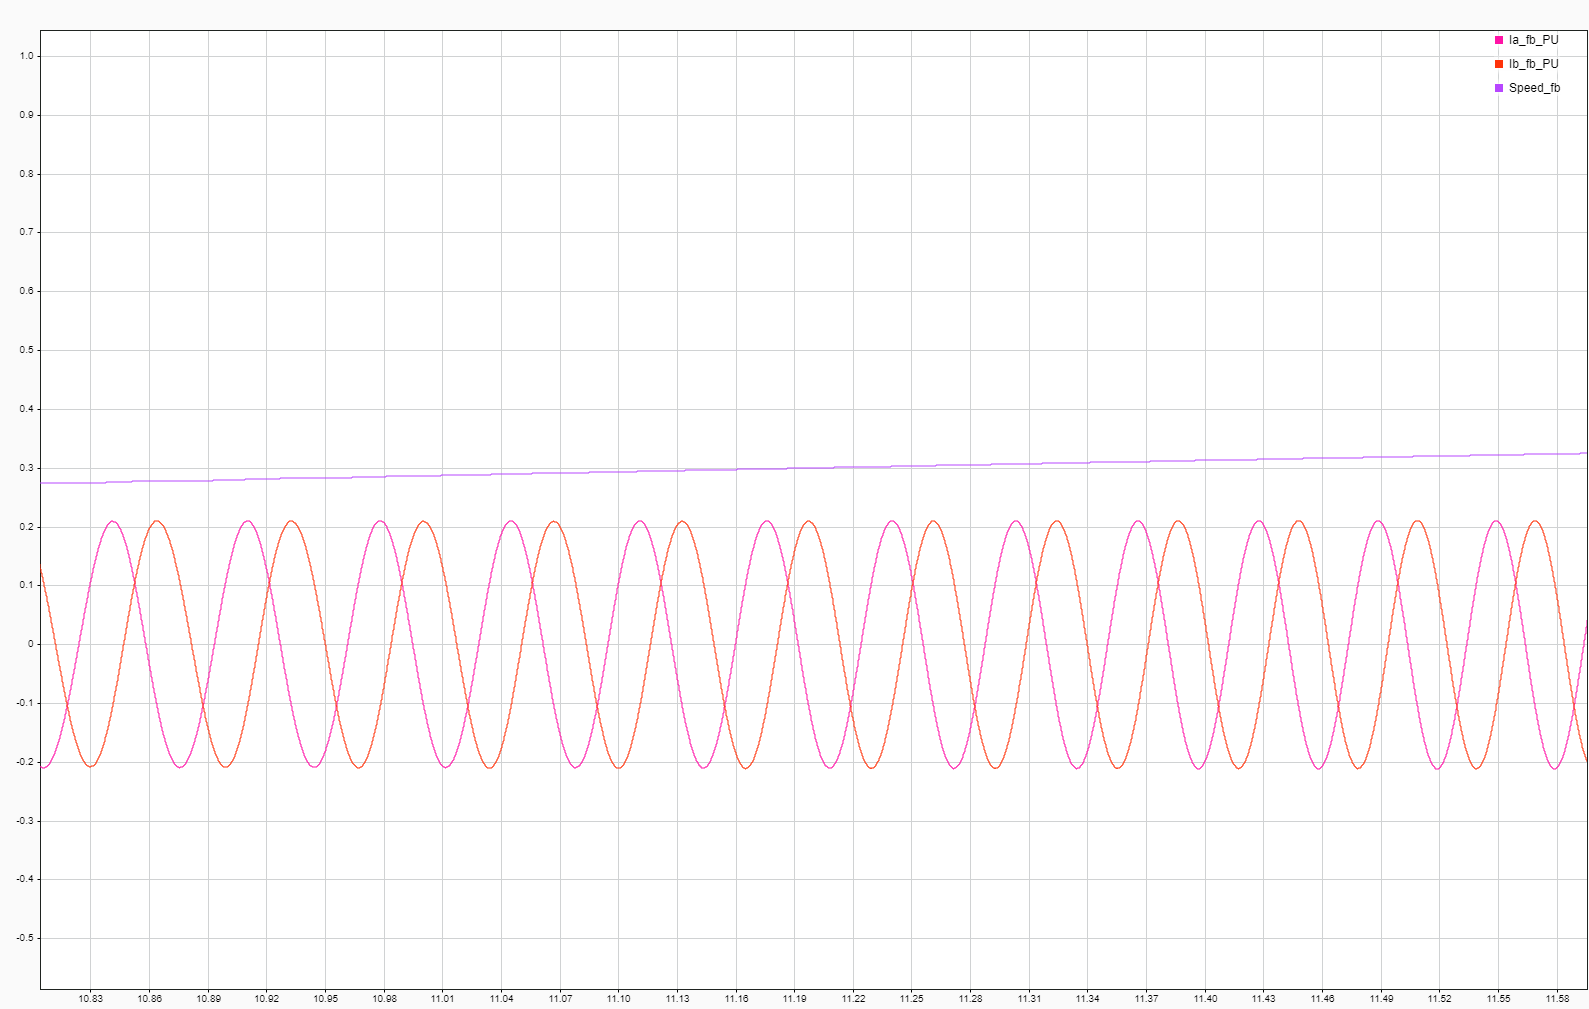
\includegraphics[width=6in]{sections/section3/images/simulationResutls/Ia_Ib_fb.png}
	\caption{Ia and Ib Feedback/Measured Currents}
	% \label{fig:current_response }
\end{figure}


\begin{figure}[H]
	\centering
	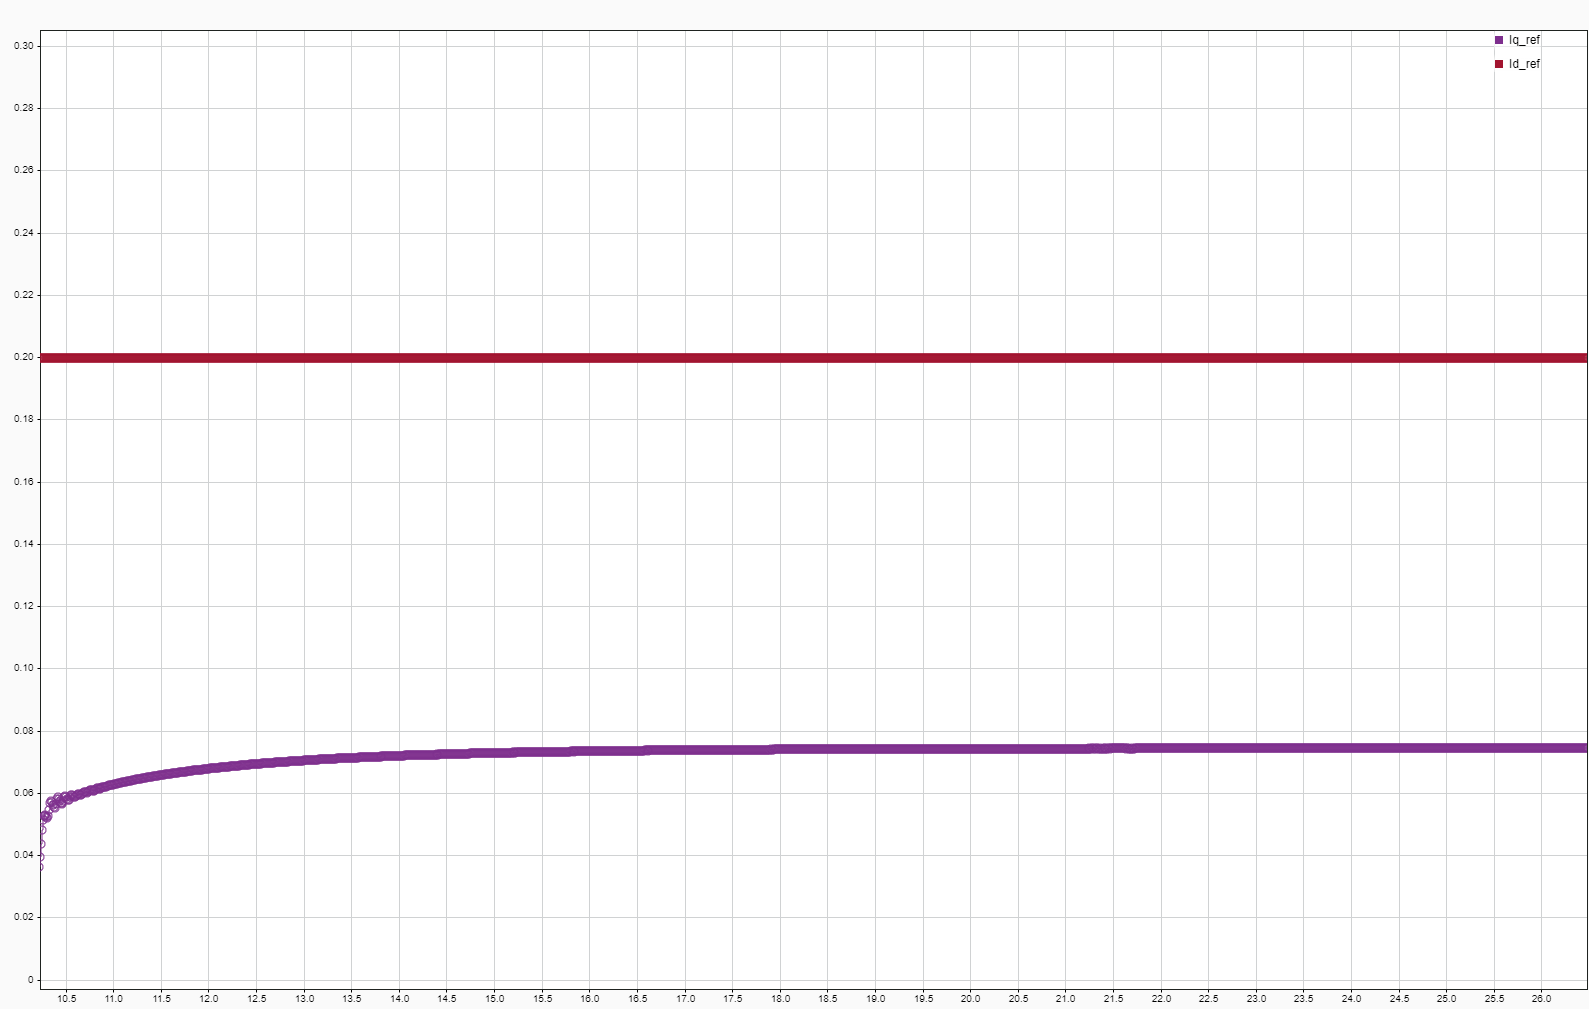
\includegraphics[width=6in]{sections/section3/images/simulationResutls/Id_ref_Iq_ref.png}
	\caption{Id and Iq Reference Currents}
	% \label{fig:current_response }
\end{figure}


\begin{figure}[H]
	\centering
	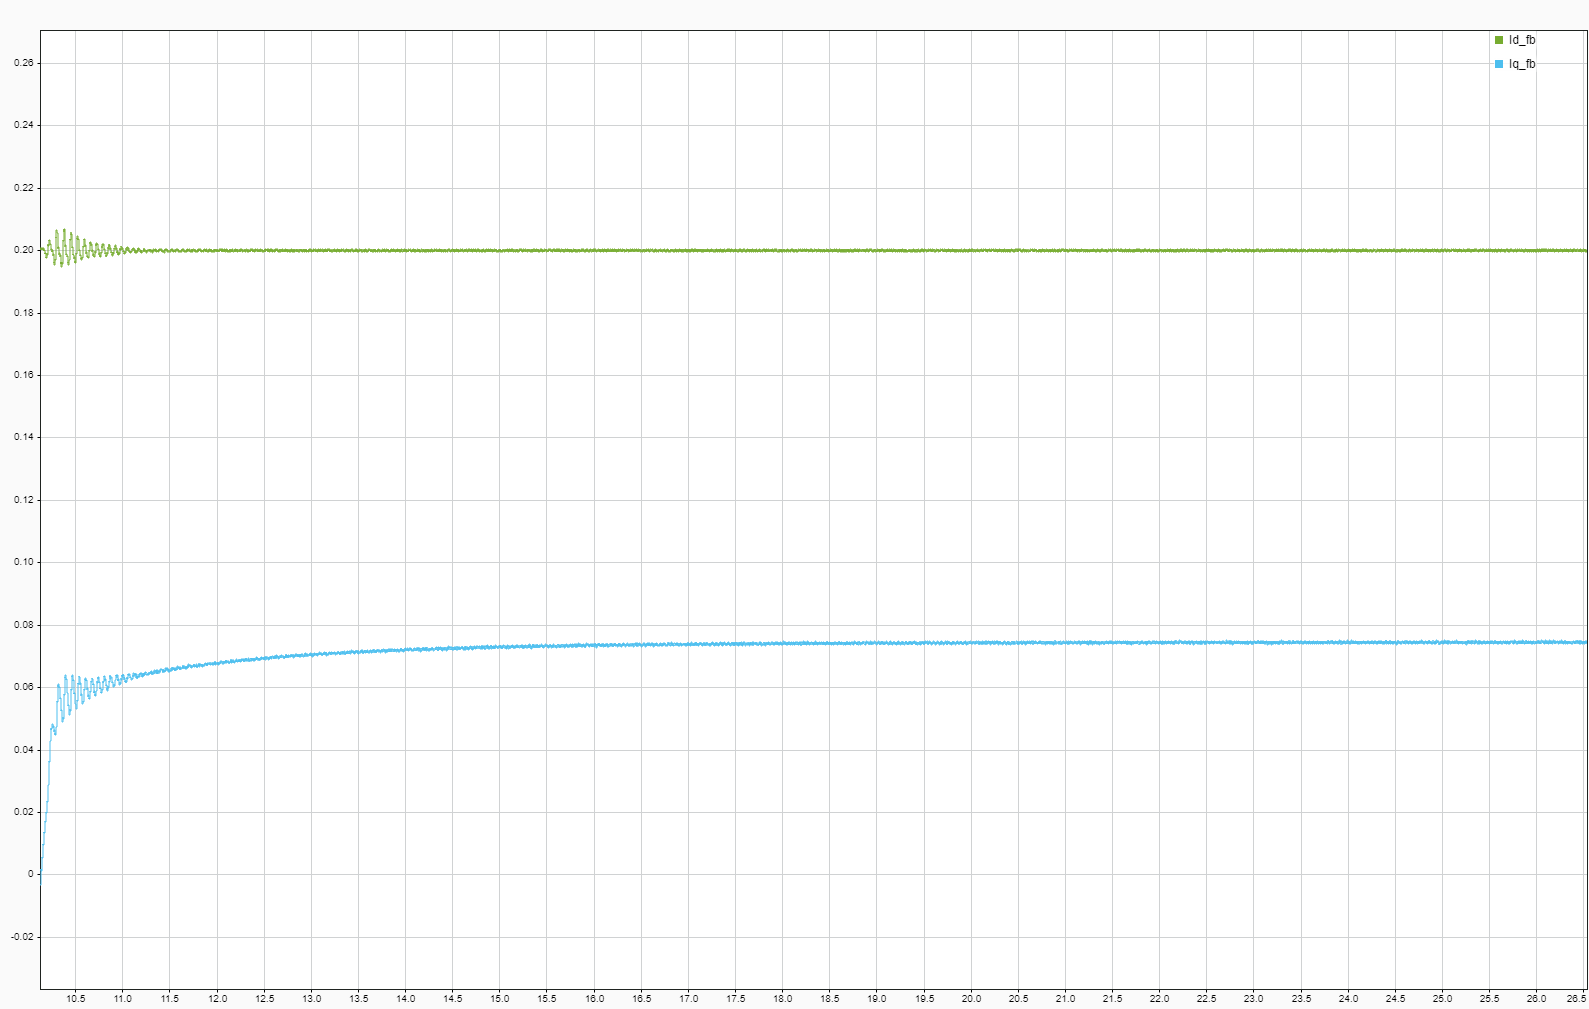
\includegraphics[width=6in]{sections/section3/images/simulationResutls/Id_fb_Iq_fb.png}
	\caption{Id and Iq Feedback Currents}
	% \label{fig:current_response }
\end{figure}

\begin{figure}[H]
	\centering
	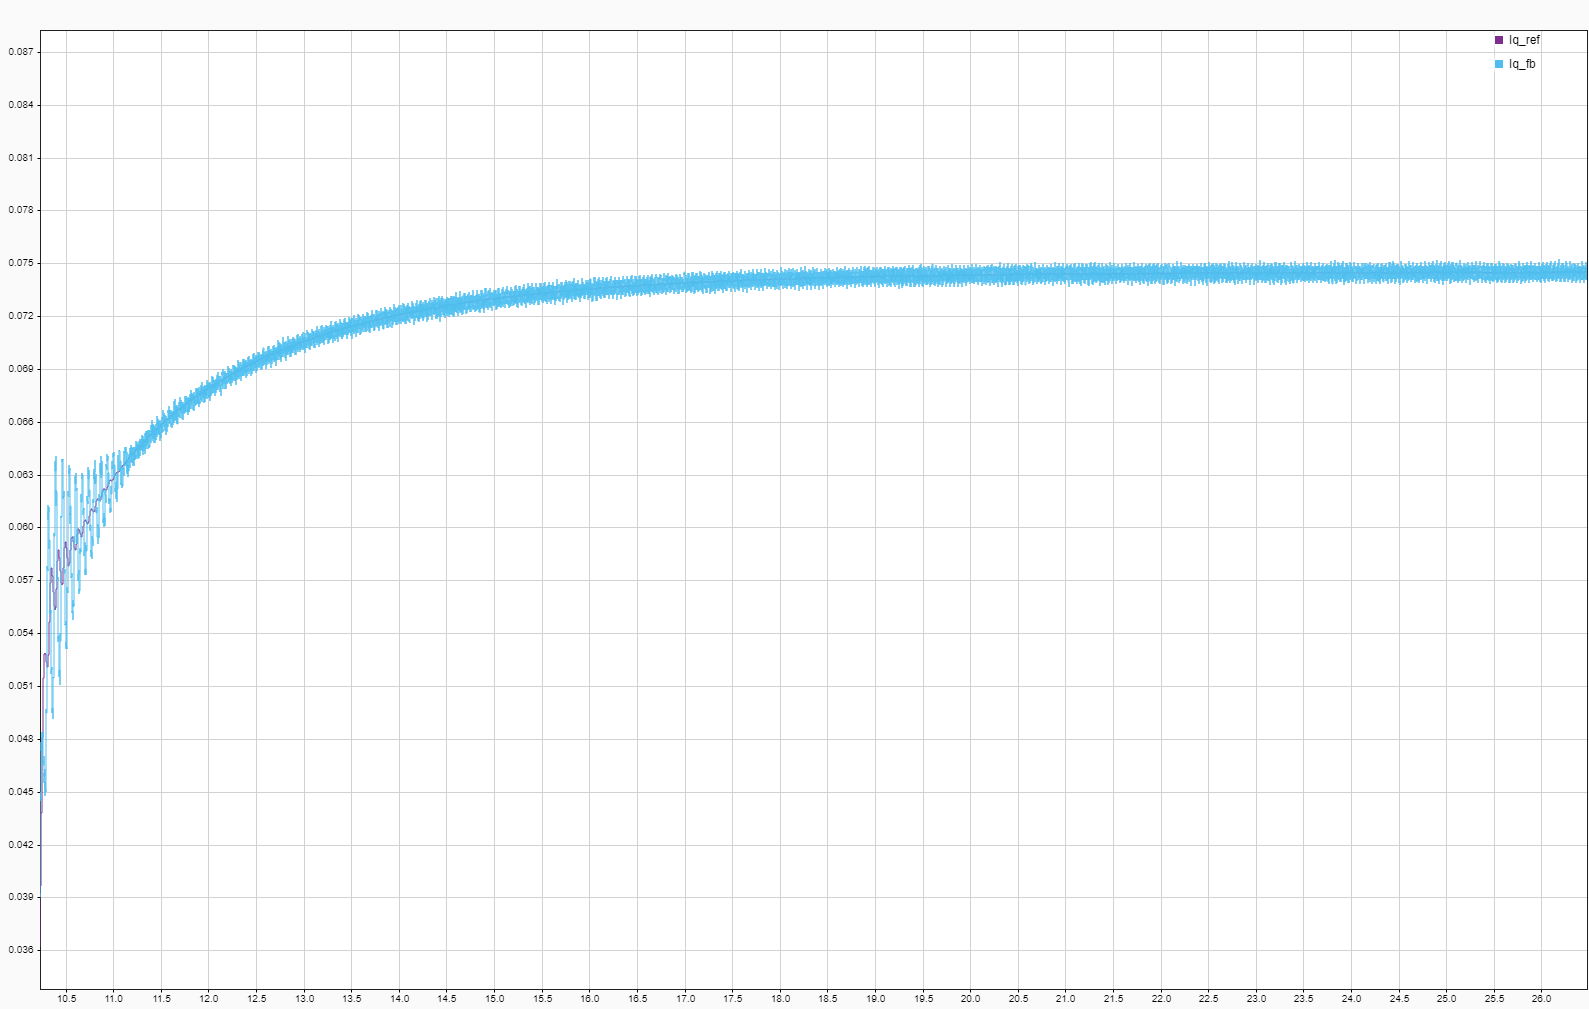
\includegraphics[width=6in]{sections/section3/images/simulationResutls/Iq_ref_fb.png}
	\caption{Iq Reference and Feedback Currents (Torque producing current)}
	% \label{fig:current_response }
\end{figure}

\begin{figure}[H]
	\centering
	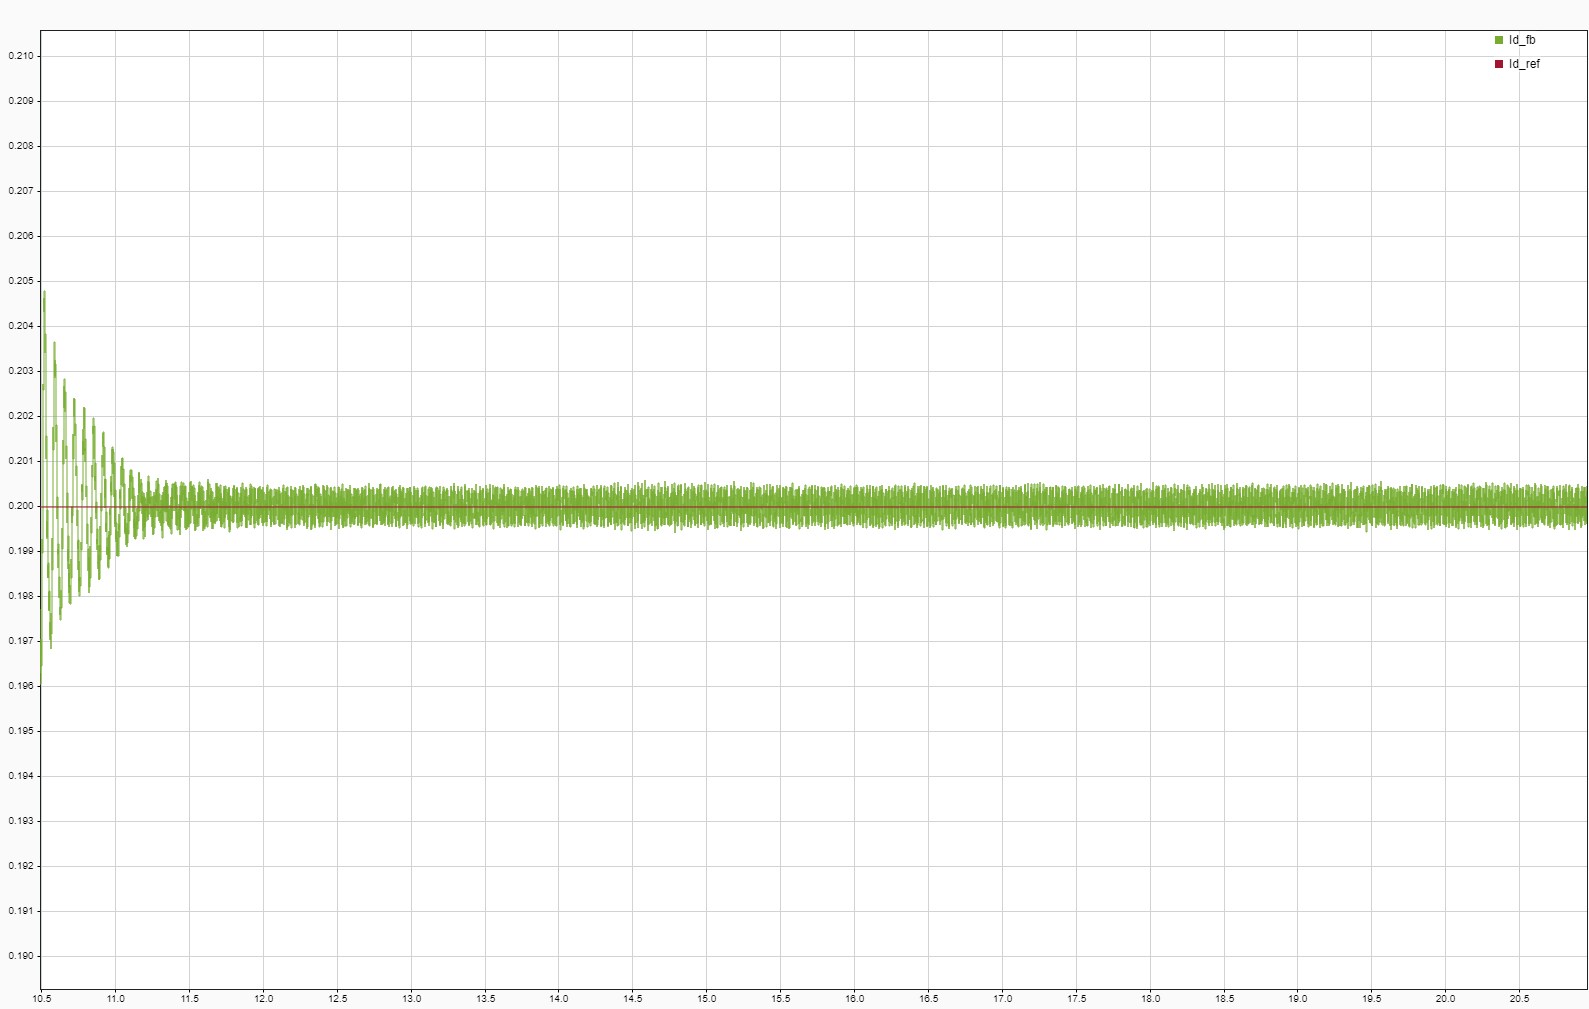
\includegraphics[width=6in]{sections/section3/images/simulationResutls/Id_ref_fb.png}
	\caption{Id Reference and Feedback Currents (Magnetizing current)}
	% \label{fig:current_response }
\end{figure}

\subsection{Chapter summary}

This chapter presented the simulation results FOC control system for an AC induction motor. The simulation was structured to validate various subsystems including speed control, current measurement, position and speed estimation, and the overall control system. Each section provided detailed insights through block diagrams and response graphs to illustrate the system's performance under simulated conditions.

\subsection{Key Findings}

\begin{itemize}
    \item The \textbf{Speed Control Subsystem} effectively managed the motor's speed by adjusting the torque reference values, ensuring that the motor speed follows the set reference closely.
    \item The \textbf{Current Control Subsystem} demonstrated robust performance in tracking the reference currents accurately, which is crucial for the stability and efficiency of the motor operation.
    \item \textbf{Position and Speed Estimation} techniques were validated to show precise estimation of the motor's speed and position, which are critical for the effective vector control of the AC induction motor.
    \item The overall system showed a \textbf{high degree of accuracy and responsiveness} in the speed and current responses, validating the effectiveness of the designed control strategies in managing the dynamics of the AC induction motor.
\end{itemize}

In conclusion, this chapter has laid a solid foundation for the practical implementation of the control system, with simulation results strongly supporting the theoretical designs.


\newpage